\chapter{Le pendule}
Un pendule simple est un système idéalisé constitué d'une masse ponctuelle suspendue à l'extrémité d'un fil inélastique de masse négligeable.

L'étude du pendule offre un bel exemple de la validité des lois en physique : le plus souvent, celles-ci ne sont vraies que dans certaines conditions et il en existe des formulations plus générales, mais plus complexes.

Un exemple célèbre est celui des phénomènes relativistes comme l'augmentation de la masse inertielle en fonction de la vitesse : \(m=\frac{m_0}{\sqrt{1-\frac{v^2}{c^2}}}\). La masse des corps est généralement considérée comme constante, mais il s'agit d'une simplification valable pour des vitesses petites par rapport à celle de la lumière.

Considérer que le mouvement d'un pendule est un MSH est une simplification qui n'est valable que pour les petits angles, cette limitation est connue comme \enquote{\motcle{l'approximation des petits angles}}.

\newpage

\section{Approximation des petits angles}
Les graphiques ci-dessous présentent les fonctions \textcolor{OliveGreen}{\(f(x)=x\)} et \textcolor{red}{\(g(x)=sin(x)\)}.

\begin{figure}[ht!]
    \begin{minipage}{.5\textwidth}
        \centering
        \begin{tikzpicture}[scale=0.55]
            \tikzset{>=latex}
            \tikzstyle{every node}=[font=\tiny]
            \tkzInit[xmin=-2,xmax=3,ymin=-2,ymax=3,xstep=0.5,ystep=0.5]
            \tkzGrid
            \tkzDrawX[label={$X$}]
            \tkzDrawY[label={$Y$}]
            %\tkzAxeXY
            \tkzAxeXY[label={}] %This macro combines the four macros: \tkzDrawX\tkzDrawY \tkzLabelX\tkzLabelYnode font=\tiny]
            \tkzFct[domain=-2:3,color=red]{sin(\x)}
            \tkzFct[domain=-2:3,color=OliveGreen]{\x}
        \end{tikzpicture}
        %\includegraphics[width=.8 \linewidth]{fonctions_x_sin_x_I.png}
        \caption{Les fonctions \(f(x)=x\) et \(g(x)=sin(x)\)}
        \label{fonctions_x_sin_x_I}
    \end{minipage}
    \begin{minipage}{.5\textwidth}
        \centering
        \begin{tikzpicture}[scale=0.55]
            \tikzset{>=latex}
            \tikzstyle{every node}=[font=\tiny]
            \tkzInit[xmin=-0.05,xmax=0.45,ymin=-0.05,ymax=0.45,xstep=0.05,ystep=0.05]
            \tkzGrid
            \tkzDrawX[label={$X$}]
            \tkzDrawY[label={$Y$}]
            %\tkzAxeXY
            \tkzAxeXY[label={}] %This macro combines the four macros: \tkzDrawX\tkzDrawY \tkzLabelX\tkzLabelYnode font=\tiny]
            \tkzFct[domain=0:.5,color=red]{sin(\x)}
            \tkzFct[domain=0:.5,color=OliveGreen]{\x}
        \end{tikzpicture}
        \caption{Les fonctions \(f(x)=x\) et \(g(x)=sin(x)\)}
        \label{fonctions_x_sin_x_II}
    \end{minipage}
\end{figure}

On remarque que lorsque x est petit, l'écart entre \(f(x)\) et \(g(x)\) est négligeable, il est donc permis de considérer que si x est petit alors \(sin(x)=x\). En pratique, cette approximation est utilisée pour des angles inférieurs à 0,1 rad, c'est-à-dire \(6^\circ\).

\newpage

\section{Équation horaire du pendule simple}
Pour étudier le pendule simple, nous utiliserons un référentiel dont les deux axes sont toujours perpendiculaires et tangents à la trajectoire.
Dans ce système d'axes, les forces qui s'exercent sur la masse \enquote{m} sont son poids, \(\vec{F_g}\), et la traction du fil, \(\vec{T}\). Le poids peut être décomposé en \(\vec{F_{gX}}\), tangent à la trajectoire et \(\vec{F_{gY}}\) perpendiculaire à celle-ci.
On peut donc écrire que :
\begin{itemize}
    \item \(F_{gX}=m \cdot g  \cdot sin(\theta)\)
    \item \(F_{gY}=m \cdot g  \cdot cos(\theta)\)
\end{itemize}



La force qui rappelle la masse vers sa position d'équilibre est \(\vec{F_{gX}}\), donc :
\begin{align}
    F(t)=F_{gX}=m \cdot g \cdot sin(\theta)
\end{align}
Dans cette équation, si \(\theta <<<\), alors \(sin(\theta)=\theta\) et donc :
\begin{align}
    F(t)=m \cdot g \cdot \theta
\end{align}


\begin{figure}[ht!]
    \centering
    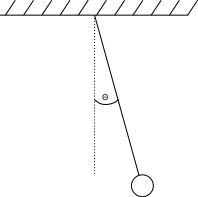
\includegraphics[width=.5 \linewidth]{demo_pendule.png}
    \caption{Les forces agissant sur un pendule simple}
    \label{demo_pendule_I}
\end{figure}

\newpage

Pour pouvoir aller plus loin, il faut exprimer l'écartement par rapport à la position d'équilibre en fonction de l'élongation et non en fonction de \(\theta\).
Pour cela, nous allons utiliser une autre approximation.
Si \(\theta\) est petit, alors l'élongation \enquote{y} peut être approximée par la longueur de l'arc OM (voir \cref{fig:demo_pendule_II} \cpageref{fig:demo_pendule_II}).
Dès lors :
\begin{equation}
    y=L \cdot \theta \ \rightarrow \ \theta=\frac{y}{L}
\end{equation}
L'équation de la force engendrant le MSH devient donc :
\begin{align}
    F(t)=m \cdot g \cdot \frac{y}{L} \rightarrow \\
    F(t)=\frac{m \cdot g}{L} \cdot y
\end{align}

On retrouve alors la structure d'une équation du MSH : une force proportionnelle à une élongation.
Dans cette équation, la constante du MSH vaut :
\begin{equation}
    \label{eqn:k_msh_I}
    k_{MSH}=\frac{m \cdot g}{L}
\end{equation}
Étant donné que l'impulsion vaut :
\begin{equation}
    \label{eqn:k_msh_II}
    k_{MSH}=m \cdot \omega^2
\end{equation}
On peut égaler ces deux équations (\ref{eqn:k_msh_I} et \ref{eqn:k_msh_II}) pour obtenir :
\begin{equation}
    \frac{m \cdot g}{L} = m \cdot \omega^2
\end{equation}

On voit que la masse se simplifie et qu'on obtient :
\begin{align}
    \omega^2=\frac{g}{L}
\end{align}

Conclusion : l'impulsion d'un pendule ne dépend pas de la masse, mais uniquement de la longueur du pendule.
\begin{equation}
    \tcboxmath[colback=LightBlue,colframe=blue]{\omega = \sqrt{\frac{g}{L}}}
\end{equation}


\begin{figure}[ht!]
    \centering
    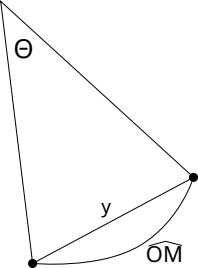
\includegraphics[width=.3 \linewidth]{demo_pendule_II.png}
    \caption{Approximation de l'élongation par l'arc de cercle.}
    \label{fig:demo_pendule_II}
\end{figure}

\newpage

\section{Exercices}
\begin{exercise}
    Un pendule effectue 30 allers-retours en 10 secondes.
    \begin{enumerate}[a)]
        \item Quelle est la longueur du pendule ?
        \item Quelle devrait être la longueur pour diviser la fréquence par 2 ?
    \end{enumerate}
\end{exercise}

\begin{exercise}
    Une balançoire est attachée à la branche d'un arbre, mais celle-ci est inclinée et forme un angle de \(20^{\circ}\). La distance entre les deux points d'attache est de 70cm et la plus petite corde de la balançoire mesure \(3[m]\).
    \begin{enumerate}[a)]
        \item Comment la balançoire va-t-elle se comporter ?
        \item La balançoire est écartée de 1[m] puis est lachée. Où se trouvent les deux points d'attache 10[s] après le premier passage par la position d'équilibre ?
    \end{enumerate}
\end{exercise}

\begin{exercise}
    Un pendule d'une longueur de 50[cm] est écarté de 4[cm] par rapport à sa position d'équlibre.
    \begin{enumerate}[a)]
        \item Quelle est sa vitesse après 10[s] ?
        \item Quelle est sa fréquence ?
    \end{enumerate}
\end{exercise}


\begin{minipage}{.5\textwidth}
    \begin{exercise}
        \qrcode{https://www.vf-bxl-moodle.be/mod/quiz/view.php?id=1441}
    \end{exercise}
\end{minipage}
\begin{minipage}{.5\textwidth}
    \begin{exercise}
        \qrcode{https://www.vf-bxl-moodle.be/mod/quiz/view.php?id=1437}
    \end{exercise}
\end{minipage}



